\documentclass[uplatex]{jsarticle}
%\documentclass[a4j]{ujarticle}
\usepackage{resume}  % resume用スタイル
\usepackage{udline}  % 下線用
\usepackage{comment} % 複数行コメント
\usepackage{multirow} % セル統合
\usepackage{makecell} % セル内で改行するため
% \usepackage{siunitx}  % 数式フォントを本文フォントにそろえるため

\pagestyle{plain}

\begin{document}
\twocolumn[
    \beginheader{令和7年度 コンピュータサイエンス学部 中間発表}{2025}{8}{7}{井上 研究室}
    \title{握り操作によるVR物体切替コントローラの提案}
    \author{C0B22045 川地 道人 (Michito Kawachi)}
    \endheader
]
\vspace{3mm}

%%ページ番号
\setcounter{page}{17}

\section{はじめに}

VRゲームをプレイする際,プレイヤーは左右にコントローラを握る.
自分のキャラクターはプレイヤーの現実での動作に同期して動く.
現実とVRとの感覚に差がないと,高い没入感を得ることができる.

コントローラも,現実との差を埋めるために有効なデバイスだ.
現実でVR内のアイテムに似せた物を持つことで,特に触覚に働きかけ,高い没入感が得られる.
しかしVRで使われるアイテムの種類が多いため,それぞれに一対一対応する専用コントローラを用意することは一般的でない.
また,専用コントローラを用意できたとしても,現在把持しているコントローラを放し,別のコントローラを探して持つことは,ゲーム体験を中断させる.

そこで1つのコントローラで多くのアイテムに対応できるデバイスが研究されてきた.


\section{関連研究}

Gonzalez らはアイテムの形状を触覚提示できるデバイスとして,X-Rings(\figref{fig:X-Rings})を提案した\cite{gonzalez2021x-rings}.
X-Ringsは手全体で握れるデバイスで,5.5cmから7.7cmに拡張可能なリングが4つ積み重ねられている.
それぞれが自由に変形するため,コップの形状やくびれのあるボトルの形状など,1つのデバイスで幅広いアイテムの触覚を提示することができる.
しかし,システムにより形状を変化させるだけで,ユーザが自由に太さを変化させることはできない.
本研究ではユーザからの入力が主体となるため,X-Ringsでは太さによるアイテム切り替えができない.

\begin{figure}[htbp]
    \centering
    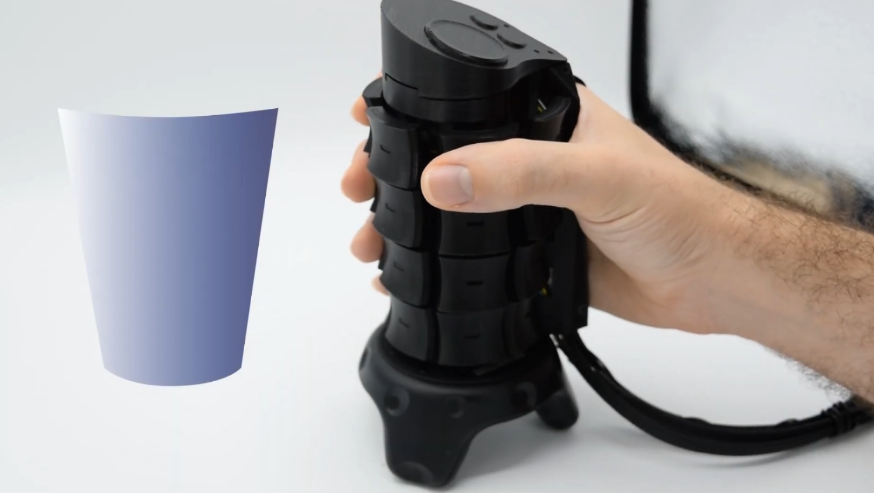
\includegraphics[width=0.9\linewidth]{fig/X-Rings.png}
    \caption{コップの形状を再現するX-Rings}
    \label{fig:X-Rings}
\end{figure}

市川らは,アイテム選択の簡略化と現実とVRでのアイテムの把持状態を一致させることを目的として,ConcateRoller(\figref{fig:ConcateRoller_concate})を提案した\cite{市川2025ConcateRoller}.
ConcateRollerは,左右で把持するコントローラを合体・分離する機構を有し,両手で操作するアイテムと片手で操作するアイテムの切り替えをメニュー操作を介さず行えるコントローラである.
% ConcateRollerを既存の汎用コントローラに取り付け,縦に合体させることで,現実とVRでのアイテムの把持形態を一致させる.
% 合体状態では両手で操作するアイテムだけを,分離状態では片手で操作するアイテムだけが選択肢に取ることができる.
プレイヤー体験に関する実験の結果,ConcateRollerを使ったアイテム切り替えにおいて,体験に与える影響の有無は有意に示されなかった.
これはConcateRollerを合体させる動きがスムーズにできないからだと考察している.
% VRと現実の把持形態の一致を目的としているが,アイテムの持ち手の太さを提示することは扱っていない.
現実で両手持ちする物体は,頭パーツが重いため,両手持ちする理由があり,持ち手が太く丈夫に作られている.
しかしConcateRollerは持ち手が細い片手用のアイテムと,太い両手用のアイテムとで持ち手の太さの差を提示できていない.

\begin{figure}[htbp]
    \centering
    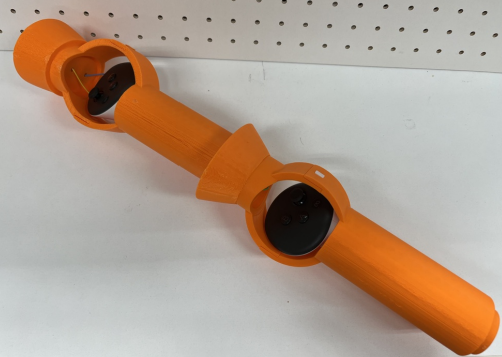
\includegraphics[width=0.9\linewidth]{fig/ConcateRoller合体.png}
    \caption{ConcateRollerの合体状態}
    \label{fig:ConcateRoller_concate}
\end{figure}

\section{握り操作により持つアイテムを切り替えるコントローラ}

\subsection{システム概要}

\figref{fig:Zentai}にコントローラの全体を示す.
図の左側はコントローラが一番太いときを表し,右側はコントローラが2番目に太いときを表す.
さらに細い1段階を加え,3段階の太さで操作する.
このコントローラは4本の円柱で太さを提示する.
\figref{fig:Zentai}中の紫色の部分だ.
ユーザが紫の円柱を握り,中心にスライドさせることで,太さを変化させられる.

\begin{figure}[htbp]
    \centering
    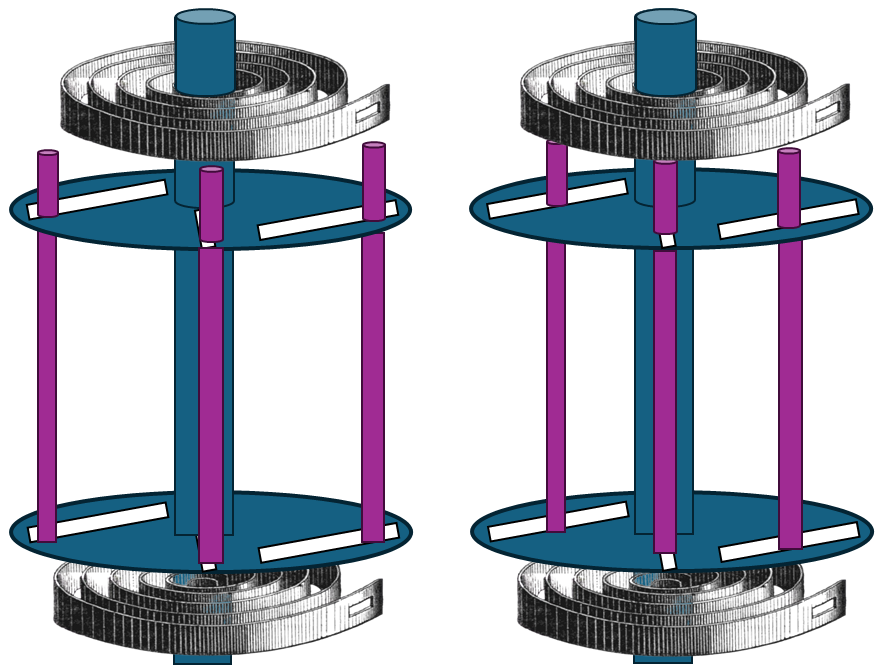
\includegraphics[width=0.9\linewidth]{fig/横からみた図.png}
    \caption{コントローラの全体}
    \label{fig:Zentai}
\end{figure}

\figref{fig:SlashGear}にユーザが握る円柱を支える円盤構造を示す.
中心の円はコントローラを貫く中心軸を,4つの紫の円はユーザが握る部分(以下4本柱)を表す.
白い部分は円盤に穴が開いていることを表す.
4本柱は円盤の穴に沿って動く.
それぞれ中心軸に対して放射状に移動する.

一番太い状態から2番目に太い状態になるときの変化を例に,4本柱の動きを説明する.
ユーザが4本柱を握って細くしようとすると,レーンの切り欠きがない面に押し付けられるように滑る.
円盤は固定されていないため,反時計回り方向に回転する.
このとき,中心軸に固定されたゼンマイばね(\figref{fig:Zentai}の上部と下部にある銀色のパーツ)が圧縮され,一番太い状態への復元力が蓄積される.
中心軸から遠い切り欠きを少し通り過ぎてから手を緩めると,ゼンマイばねの復元力によって,円盤が時計回りに回転する.
4本柱が中心軸から離れるようにレーンに押され,中心から遠い方の切り欠きに引っ掛かりロックされる(\figref{fig:SlashGear}の中央).

\begin{figure}[htbp]
    \centering
    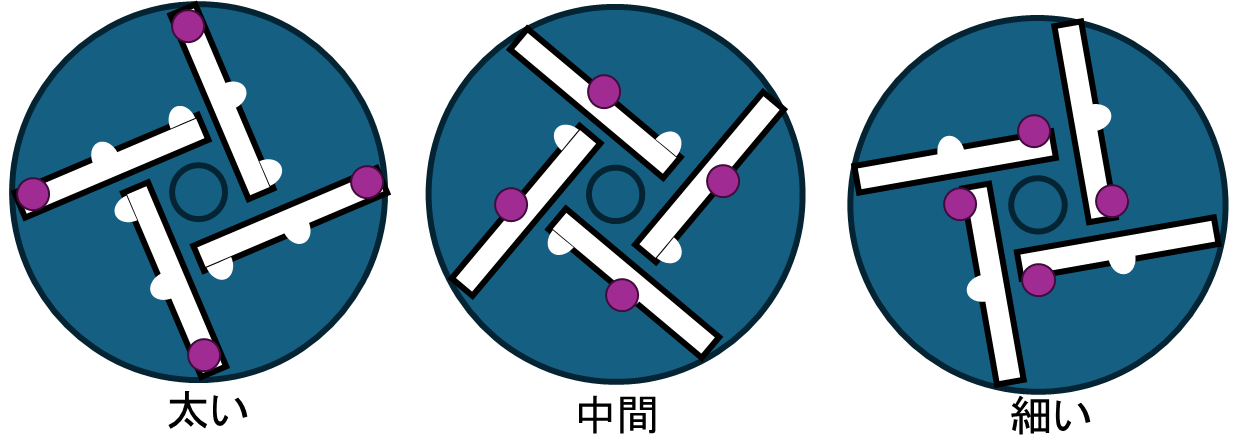
\includegraphics[width=0.9\linewidth]{fig/太さ3段階.png}
    \caption{太さを変更する機構}
    \label{fig:SlashGear}
\end{figure}

% 上下のゼンマイばねによって4本柱に常に外側に戻る方向の力が働くため,この機構は太さ変更のために電子部品を必要としない.
機構の検討事項を示す.
1つ目は現在の太さの検知方法だ.
ロータリーエンコーダを使う方法と,切り欠きのロック部分と,4本柱のロック機構と同じ高さに銅箔テープを巻き,接触しているかで検知する方法の2つを検討している.
2つ目はロック機構の解除方法だ.
現状4本柱を同じ太さにとどめる機構は提案できたが,ロックを解除する方法については考慮が必要だ.
切り欠きから内側に力を与える方法か,切り欠きを埋めるパーツで押し出す方法の2つを検討している.

\subsection{システム構成}

システム構成を\figref{fig:system}に示す.
コントローラの現在の太さをPCに入力し,VRプレイヤーのアイテムを対応する太さのアイテムに切り替える.
また,コントローラとPCは無線接続を検討している.
ユーザが自由に動かせることで没入感に影響すると考えたからだ.

\begin{figure}
    \centering
    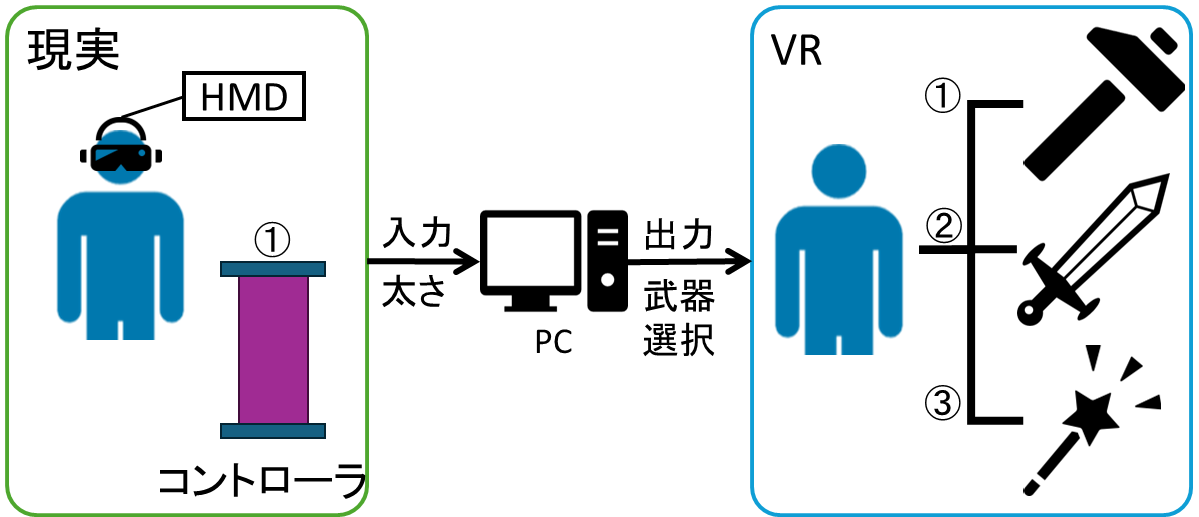
\includegraphics[width=0.9\linewidth]{fig/構成図.png}
    \caption{システム構成}
    \label{fig:system}
\end{figure}


\section{評価方法}

ユーザにHMDとコントローラを装着させ,指定された武器で目標を切ってもらう実験を実施する.
武器の選択方法を提案手法と既存のVRコントローラを使う方法の2種類についてそれぞれ行う.
被験者は,実験後没入感や使いやすさに関するアンケートに回答する.

武器の切り替えにかかった時間,武器を間違えて攻撃した回数,タスクにかかった時間などの定量評価と,没入感や使いやすさ,掌から感じた太さと視覚から感じた太さの乖離などについて,5段階のリッカートスケールで評価する.

\section{まとめ}

本研究では,持ち手の太さでアイテムを切り替えられる操作手法の提案した.
視覚と触覚の差を埋めることで,没入感の高いコントローラを開発できると考えている.



\bibliographystyle{junsrt}
\bibliography{ref}

\end{document}